
%%%%%%%%%%%%%%%%%%
%%% EVALUATION %%%
%%%%%%%%%%%%%%%%%%

\chapter{Evaluation}
\label{evaluation}

This chapter presents an evaluation of the solution designed in chapter~\ref{design}, by way of a usability study of the TIDE prototype.
The evaluation focuses on three system aspects: learnability, ease of use and usefulness.

The methods used are based on Designing Interactive Systems by
\cite{Benyon:2010}, and described in section~\ref{sec:methods}.
The evaluation results are presented in section~\ref{sec:results}.

\section{Parameters}
\label{sec:parameters}

To demonstrate that the solution proposed is valid,
this evaluation shows that TIDE allows spontaneous user interaction, and that it is a useful application.
The evaluated parameters are the system's learnability and ease of use, that are major aspects of usability; and the system's usefulness.

\begin{description}
\item[Learnability] is the capability of a software product to enable the user to learn how to use it.
%It is evaluated by engaging end users in an exploratory interaction with the system, and assessing whether this is sufficient for users to learn how to use it.

\item[Ease of use] is the self-perceived level of effort that the use of a software product requires of the user.

\item[Usefulness] is the quality of being useful, and a requirement for user satisfaction.
%It is evaluated here by asking end users to assess whether they would use the application in specific situations.

\end{description}

\subsection{Variables}

The six \emph{interaction primitives} that were defined in section~\ref{sec:strategies} are independent variables.
They are the application features that are implemented by TIDE, and the minimum set of features to allow a successful user interaction.
However, only five primitives were evaluated: \emph{dragging, rotating, resizing, minimizing and closing}.
The sixth primitive, \emph{hiding}, was removed, due to user feedback from the design process that showed it was similar, if not interchangeable, with minimizing.
\\
\linebreak
The interaction techniques that were implemented as a result of the design decisions from section~\ref{sec:design} are dependent variables.
The goal of this evaluation is to discover which of these interaction techniques are intuitive to the user and which ones the user prefers. 

%Another dependent variable is the usefulness of the system, assessed by end-users during this evaluation.

\section{Methods}
\label{sec:methods}

Given the strong focus of the present work on user interaction, it was decided to use participant-based methods to evaluate the system.
A usability study involving end-users was designed, that regrouped the selected methods in one experiment session.

\begin{description}

\item[Discovery]

To evaluate learnability, users are engaged in discovering the system on their own.
With no prior knowledge of the application, participants are given three minutes to \emph{learn by doing}, i.e.\ explore the system without exterior help.
Qualified data is gathered to evaluate how much of the system the users were able to learn.

\item[Guided test]

To evaluate ease of use, a semi-controlled experiment is designed.
Participants are asked to perform specific tasks using the system.
Detailed instructions are given to the user during the test.
These instructions mention only the independent variables, and the behavior of the user provides data to evaluate the dependent variables.
In the present case, the instructions only address the interaction primitives, and it is up to the user to choose between the available interaction techniques.
Qualified data is gathered to evaluate the dependent variables.

\item[Questionnaire]

A questionnaire is used to gather data that supports the evaluation of all three parameters.
Participants are asked to assess the learnability, ease of use and usefulness of the system by answering carefully designed questions.

\end{description}


\section{Experiment}
\label{sec:experiment}

In order to generate qualified data, a user experiment was designed and conducted.
Figure~\ref{fig:andrea} shows a participant during an experiment session.

\subsection{Participants}

Thirteen participants aged between 25 and 40 were recruited on a voluntary basis.
Five out of the thirteen had no technical background, and three out of those five were female participants.
All were regular smartphone users.

\begin{figure}[htb]
  \centering
    \includegraphics[width=1\textwidth]{images/tideandrea}
    \caption{A volunteer using the TIDE prototype.}
    \label{fig:andrea}
\end{figure}

\subsection{Apparatus}

The experiment sessions were carried out at the PITLab (Pervasive Interaction Technology) at the IT University of Copenhagen.
The TIDE prototype was installed on the Microsoft Surface tabletop computer, and used in combination with an iPhone 4 and a HTC Legend smartphone, both equipped with third-party VNC applications.
A additional desktop computer was available for filling out online evaluation forms.

\subsection{Procedure}

A session lasts 30 minutes, and involves a participant and the designer.
The session is structured by an experiment script, included in appendix~\ref{app:evalscript}, that is read by the designer to the user.

First, the participant is introduced to the following things:
\begin{itemize}
\item the structure of the session (a discovery phase, a guided test and a questionnaire),
\item the devices (Microsoft Surface, iPhone and HTC Legend);
\item the TIDE prototype:
	\begin{itemize}
	\item the pairing procedure,
	\item the lack of responsiveness of the replicated UI,
	\item the difference between the replicated UI and the surface UI;
	\end{itemize}
\item the fact that only the system is under test, not the participant.
\end{itemize}

The participant is then taken through the following phases: discovery, guided test and questionnaire.

\subsubsection{Discovering TIDE}

The participant has been shown how to pair the phone to the Microsoft Surface.
S/he is given three minutes to freely explore the application features of the application.
At the end of this discovery phase, the designer fills out the evaluation form \emph{Tide-EF1}, included in appendix~\ref{app:evalforms}, where he records for each of the interaction primitives, which of the interaction techniques the user discovered.

\subsubsection{Testing TIDE}

In order for the participant to be able to use TIDE to its full potential, s/he is taught all the available interaction techniques before the beginning of the guided test.

The test consists of two small scenarios, that require of the participant that he performs specific tasks with the application.
The first scenario involves the user and the designer playing a game of tic-tac-toe, and the second one involves the user looking up a location on Google Maps and showing it to the designer.
The tasks are explained, and detailed instructions are given to the user during the test, but for each instruction, it is up to the user to decide which interaction technique to use.
For example, the user is told to minimize the window, but not \emph{how} to activate the command.

This test allows the user to engage several times with all the interaction primitives, each time requiring that s/he chooses a technique of choice.
For example, a given user will prefer to drag a window using two hands, while another one will rather use a single finger.

The evaluation data is gathered via the questionnaire filled out during the next phase.

\subsubsection{Answering questions about TIDE}

The participant is asked to fill out a questionnaire, the evaluation form \emph{Tide-EF2}, included in appendix~\ref{app:evalforms}.
The user is asked to express an opinion about the following things:
\begin{itemize}
\item which interaction techniques are his/her favorites?
\item is the application easy to learn, easy to use, useful?
\item what is best/worst/missing in the application?
\item in which situations would the application be useful? 
\end{itemize}

%\subsection{Data}

The evaluation data was gathered via the aforementioned forms, then converted to excel files to be processed.
% as well as application logging.
The data was processed manually, analyzed, and results were derived.
%Additional data was generated through runtime logging during the application sessions.
%The logging data was not used to derive conclusive results, but to confirm the findings presented hereunder. 

\clearpage
\section{Results}
\label{sec:results}

Qualified data was generated via the previously mentioned forms \emph{Tide-EF1} and \emph{Tide-EF2}, included in appendix~\ref{app:evalforms}.
The forms were converted to excel files and processed manually.
The following results were derived from the analysis of the data.
They revealed that the system shows good learnability, ease of use and usefulness.
%These three system aspects were assessed by end users at the end of the experiment sessions.
\\
\linebreak
To get a general assessment of the application, the following 5-level Likert scale was used:
\begin{tightlists}
\begin{description}
\item[5] Strongly agree
\item[4] Agree
\item[3] Neither agree nor disagree
\item[2] Disagree
\item[1] Strongly disagree
\end{description}
\end{tightlists}
The answers are presented in figure~\ref{fig:evalagree}, where colored cells contain mean values above 4.
They confirm that the majority of the participants found the application easy to learn, easy to use and useful in context.

\begin{figure}[htb]
  \centering
    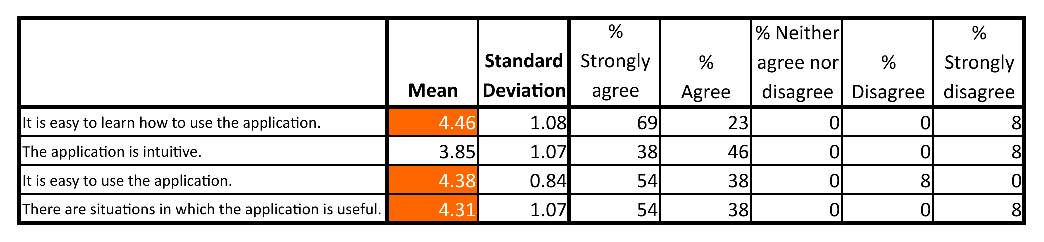
\includegraphics[width=1\textwidth]{images/evalagree}
    \caption{End users' assessment of the system's learnability, ease of use and usefulness.}
    \label{fig:evalagree}
\end{figure}

For each of the evaluated parameters, further results were derived from the experiment data.

\subsection{Learnability}

All participants were able to discover at least one technique to perform each of the necessary primitives to a successful interaction with the system.
In other words, all participants could find out on their own and within three minutes how to drag, rotate, resize, minimize and close the main application window on the tabletop.

It can thus be concluded that the system implements interaction techniques that comes naturally to most users.
Figure~\ref{fig:evaldisco} shows which specific techniques were discovered by the participants. The colored cells contain values above 50\%.
%The experiment here could have been made more interesting:
%- differentiation of ways to drag the window around (1 or 2 fingers?) 

\begin{figure}[htb]
  \centering
    \includegraphics[width=0.7\textwidth]{images/evaldisco}
    \caption{Interaction techniques that were discovered by the end users.}
    \label{fig:evaldisco}
\end{figure}

The first thing that can be remarked upon is that, although all the basic shape manipulation techniques were easily discovered, the two-handed rotating and resizing gestures scored higher than their single-handed counterpart.
This points towards the fact that it is more intuitive to perform these gestures with both hands.

Given that all participants could somehow resize the window, 85\% logically found out that they could use it to minimize it as well.
In most cases, the user stumbled upon this feature by accident, while exploring the resizing feature.
This is an example of how design can enable the user to \emph{learn by doing}.

Only 46\% of the users found out that the window could be minimized by being dragged to the edge, and none discovered the possibility of closing the window by bringing it to a corner.
These techniques were implemented because of their success among end users during the design sessions based on low-fidelity prototypes.
They were expected to be easy to discover because of their consistency with how people would interact with a document on a normal table.
However, it seems that this success was prompted by the fact that  the prototypes were actual pieces of paper, which could only be minimized/hidden/closed by being physically put away.

Similarly, none discovered that the window could be minimized by tapping it with the whole hand, even though the gesture was thought to be natural due to its resemblance to the action of hiding a document on a normal table.
It can be remarked that this gesture is not used on common devices such as smartphones or personal computers.
It is a gesture that requires a lot of space and is therefore specific to large interactive surfaces, and thus not part of the common IT knowledge of most users.

69\% of the participants found out about the double tap, which is a large amount, considering the fact that the feature is hidden, i.e.\ it can not be discovered by accident while exploring the manipulation possibilities, but has to be explicitly attempted.
It shows that, as opposed to the whole hand tap, the double tap is part of the common IT knowledge.

Pressing and holding on the window to close it is also a hidden feature, and it was discovered by none.
However, the results concerning the primitive \emph{closing} are not considered conclusive, due to the fact that users did not attempt to discover different ways to close the application during the exploratory phase, but only performed it once to terminate the session.

\subsection{Ease of use}

To determine which interaction techniques were the most efficient, participants were asked to select their favorites.
The answers are presented in figure~\ref{fig:evalfavor}, where colored cells contain values above 50\%.
This study only addresses the primitives for which multiple techniques were implemented.\footnote{Two techniques were not included in the study due to a human mistake: rotating with 1 finger and closing with press and hold.}
Participants were not limited to select one technique per primitive.

\begin{figure}[htb]
  \centering
    \includegraphics[width=0.7\textwidth]{images/evalfavor}
    \caption{End users' favorite interaction techniques.}
    \label{fig:evalfavor}
\end{figure}

It is interesting to see that users preferred to resize and rotate by using a two-handed gesture, even though it could be done single-handedly.
An explanation might be that the two-handed gesture seems to provide more control to the user, especially when s/he has little experience with touch shape manipulation on large surfaces.
%Especially since using two hands allow the user to grab the shape at both its extremities
%This is especially true given that most users had little or no prior experience with large touch screens.

To minimize, the favored techniques were double tap and the whole hand tap.
Resizing the window down to minimize it was only favored by 8\% of the users, even though it was the most easily discovered technique, whereas using a whole hand tap could not be discovered, but ended up among the most appreciated ones.
This shows that familiar and efficient features are not necessarily the same, and that both are needed.
The familiar gestures make the system easy to learn, while the efficient ones, such as the double tap or the whole hand tap, make it easy to use.

The gestures that involved dragging the window to an edge or corner of the tabletop did not score as high as expected among the participants.
The hypothesis that such gestures would be appreciated because of their consistency with normal table interaction, i.e.\ their similarity with the action of putting a document away, was not confirmed.
The first explanation that comes to mind is that a dragging gesture requires more time and space to be performed than, say, a double tap, which is quicker and can be done on the spot.


\subsection{Usefulness}

The participants expressed the opinion that the application would be useful in specific situations.
As part of the questionnaire, they were asked which activities they would consider using the system for, and in which context.
The answers are presented in figure~\ref{fig:evalcontext}, where colored cells contain values above 50\%.

\begin{figure}[htb]
  \centering
    \includegraphics[width=1\textwidth]{images/evalcontext}
    \caption{The contexts in which the application is useful.}
    \label{fig:evalcontext}
\end{figure}

The participants were presented with a list of 7 activities that could be performed on a smartphone.
For each of those activities, the users were asked first if they would use their smartphone to do them, then in which context they would consider using the application instead.
The contexts suggested were: alone in a private space, alone in a public space, together with friends or colleagues.

The results show that whether a user would choose the application or not depends mostly on privacy and trust.

The first realization is that the system is not a proper platform for activities that involve private data.
There are two activities that most users do on smartphones, but very few would do on a tabletop, whatever the context: reading and writing emails or sms messages.
Both activities involve viewing text that would potentially contain personal conversations.
It is therefore natural, that users would not want to view this data on the large open display of a tabletop.

The second realization is that there are indeed a series of activities for which the system is suitable.
They are: browsing the internet, looking at pictures, playing games and looking at a map.
However, most users would only use the application for these activities in a \emph{trusted} context, i.e.\ in a private space, or together with trusted acquaintances.
In a public context, the only activity that a majority of users would still consider doing with the system is looking up a location on a map.
Again, the explanation to this can probably be found in the fact that tabletops are very public devices, in the sense that they can be seen by any person in range.
Unlike smartphones, laptops, or even desktops, whose screen can be rotated more or less freely, tabletop displays are there for the world to see.
Thus, users are reticent to use them in public, even for semi-private occupations such as browsing the internet or playing games.

Last but not least is the realization that the system has most potential for the activity of reading documents.
It is the only activity that only a minority of users (31\%) would do on a smartphone, which confirms the hypothesis that smartphone screens are too small for this type of graphically intense data.
62\% of the participants would consider using the application for reading documents, though only in a trusted context.
Thus, the system seems to address a real need.


















